\subsection*{Mixed Cell Volume Radionuclide Transport Model}\label{sec:mixed_cell}
Slightly more complex and suited to representing waste form and buffer 
components, the mixed cell model incorporates solubility limited, congruent 
release under the influence of elemental solubility limits, sorption, diffusive 
behavior, and advective behavior. Abstraction results concerning the 
transition between primarily diffusive and primarily advective transport regimes 
were used for benchmarking and to iteratively improve accuracy in the development 
of this model.

A main nuclide transport component model used in this work is a mixed cell 
component module incorporating solubility and sorption effects as well as  
engineered material dissolution.

A graphical representation of the mixed cell model is given in Figures 
\ref{fig:intact} and \ref{fig:dissolved}.  

\begin{figure}[h!]
\begin{minipage}[b]{0.5\linewidth}
  \begin{center}
    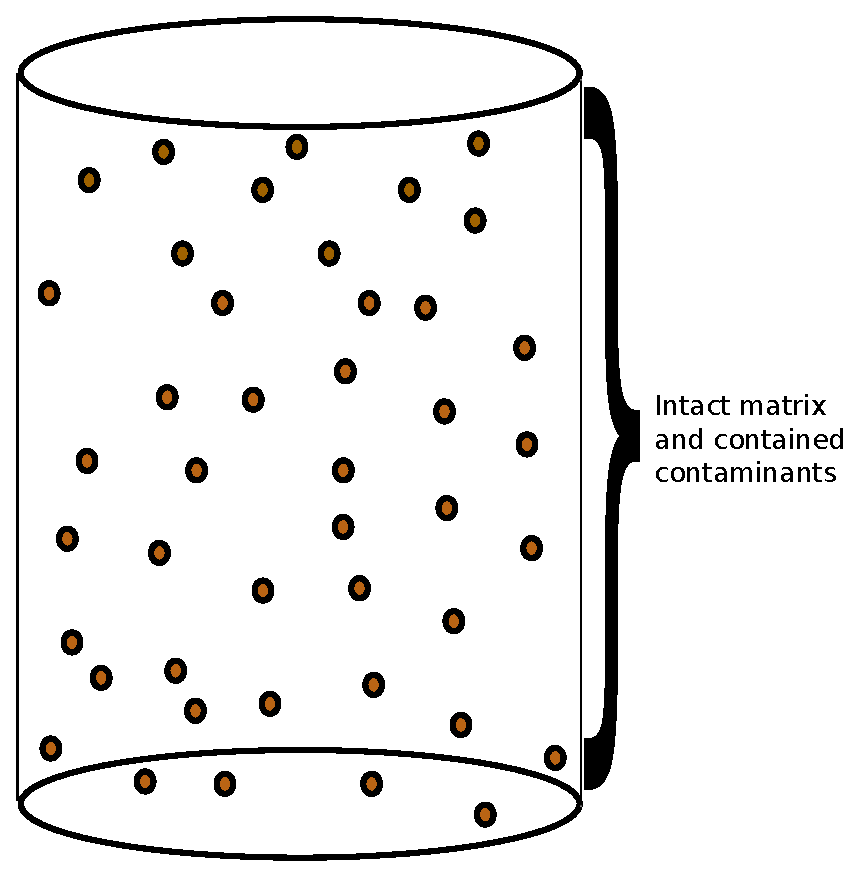
\includegraphics[width=0.9\linewidth]{mixed_cell/mixed_cell_whole.eps}
  \end{center}
  \caption[Intact Mixed Cell Control Volume]{The control volume contains an 
  intact material matrix. Contaminants are unavailable to neighboring 
  subcomponents until dissolution has begun.}
  \label{fig:intact}
\end{minipage}
\hspace{0.5cm}
\begin{minipage}[b]{0.5\linewidth}
  \begin{center}
    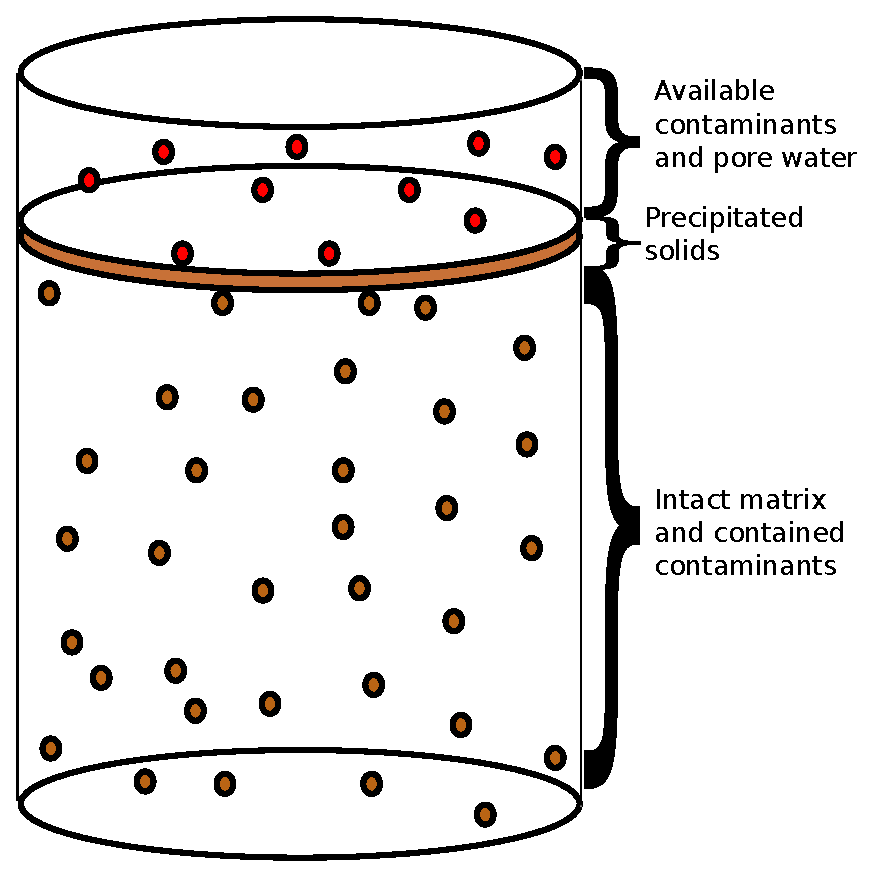
\includegraphics[width=0.9\linewidth]{mixed_cell/mixed_cell_degraded.eps}
  \end{center}
  \caption[Degrading Mixed Cell Control Volume]{Once dissolution begins, the 
  control volume contains a partially dissolved material matrix, contaminated 
  pore water, and precipitated solids.}
  \label{fig:dissolved}
\end{minipage}
\end{figure}


After some time degrading, the volume of free fluid can be expressed as
\begin{align}
V_{ff}(t_n) &= \theta V_T \int_{t_0}^{t_n} f(\cdots) dt.
\label{vff}
\end{align}

The volume of the intact matrix can be expressed as
\begin{align}
V_{im}(t_n) &= V_T - V_T\int_{t_0}^{t_n} f(\cdots) dt.
\label{vim}
\end{align}

Finally, the volume of the precipitated solids can be expressed as
\begin{align}
V_{ps}(t_n) &= (1 - \theta)V_T\int_{t_0}^{t_n} f(\cdots) dt.
\label{vps}
\end{align}

This model assumes that all net influx to the cell enters the free fluid rather 
than the intact matrix. The total volumetric contaminant concentration in the intact matrix, 
can be expressed as

\begin{align}
C_{im}(t_n) &= C_0\\
            &= \frac{m_0}{V_{im}(t_0)}
\intertext{where}
%here we assume nothing escapes an intact matrix
m_0 &= \mbox{ total initial mass. } \nonumber
\end{align}

The resulting contaminant mass in the intact matrix at time $t_n$ is 

\begin{align}
m_{im}(t_n) &= C_0 V_{im}(t_n)\nonumber\\
            &= C_0V_T\left(1-\int_{t_0}^{t_n}f(\cdots)dt\right). 
\label{mim}
\end{align}

The contaminant mass in the free fluid is just the initial pore water concentration 
times the free fluid volume plus the time integral of net influx to the cell
such that

\begin{align}
C_{ffT}(t_n) &= \left[C_0 + \frac{\int_{t_0}^{t_n} \dot{m}_{i}(t') dt'}{V_{ff}(t_n)}\right] 
\intertext{and}
m_{ffT}(t_n) &= C_{ff}(t_n) V_{ff}(t_n)\nonumber\\
       &= \left[C_0 + \frac{\int_{t_0}^{t_n} \dot{m}_{i}(t') dt'}{V_{ff}(t_n)}\right] V_{ff}(t_n) \nonumber\\
       &= C_0V_{ff}(t_n) + \int_{t_0}^{t_n} \dot{m}_{i} dt'.
\end{align}

It is limited, however, by both solubility limitation and sorption. 

\subsubsection*{Sorption}

The mass in both the free fluid and in the intact matrix exists in both 
sorbed and non-sorbed phases. The relationship between the sorbed mass 
concentration in the solid phase (e.g. the pore walls),

\begin{align}
s &=\frac{\mbox{ mass of sorbed contaminant} }{ \mbox{mass of total solid phase }}
\label{solid_conc}
\end{align}
and the dissolved liquid concentration, 
\begin{align}
c &=\frac{\mbox{ mass of dissolved contaminant} }{ \mbox{volume of total liquid phase }}
\label{liquid_conc}
\end{align}
can be expressed by a number of isotherm models.

In this model, sorption is taken into account throughout the volume. In the 
intact matrix, the contaminant mass is distributed between the pore walls and 
the pore fluid by sorption.  So too, contaminant mass released from the intact 
matrix by degradation is distributed between dissolved mass in the free fluid 
and sorbed mass in the precipitated solids.

To solve for the boundary conditons in this model, the amount of non-sorbed 
contaminant mass in the free fluid must be found. This value, $m_{ffl}$, can be 
expressed in terms of the total degraded contaminant mass and the contaminant 
mass in the precipitated solid,

\begin{align}
m_{ffl} &= m_{ffT} - m_{psc}.
\label{m_ffl}
\end{align}

The mass of contaminant sorbed into the precipitated solids can be found using a 
linear isotherm model \cite{schwartz_fundamentals_2003}, characterized by the relationship 
\begin{align}
s_{i} &= K_{di} c_{i}
\label{linear_iso}
\intertext{where}
s_i &= \mbox{ the solid concentration of isotope i }[kg/kg]\nonumber\\
K_{di} &= \mbox{ the distribution coefficient of isotope i}[m^3/kg]\nonumber\\
c_i &= \mbox{ the liquid concentration of isotope i }[kg/m^3].\nonumber
\end{align}

Thus, from \eqref{solid_conc},

\begin{align}
s_{i,ps} &= \frac{\mbox{contaminant mass in precipitated solids} }{ \mbox{total mass of precipitated solids}}\nonumber\\
         &= \frac{m_{psc}}{m_{psT}}\nonumber\\
         &= \frac{m_{psc}}{m_{psm} + m_{psc}}\nonumber
\intertext{where}
m_{psm}  &= \mbox{ noncontaminant mass in precipitated solids }[kg]\nonumber\\
         &= \rho_bV_{ps}\nonumber\\
m_{psc}  &= \mbox{ contaminant mass in precipitated solids }[kg]\nonumber\\
\rho_b   &= \mbox{ bulk (dry) density of the medium }[kg/m^3].\nonumber\\
\end{align}

The following expression results, giving contaminant mass in the precipitated 
solids in terms of the sorption coefficient,
\begin{align}
m_{psc} &= s_{ps}m_{psT}\nonumber\\
          &= K_dC_{ffl}m_{psT}\nonumber\\
          &= \frac{K_dm_{ffl}m_{psT}}{V_{ff}}\nonumber\\
          &= \frac{K_d}{V_{ff}}(m_{ffT}-m_{psc})m_{psT}\nonumber\\
          &= \frac{K_d}{V_{ff}}(m_{ffT}-m_{psc})(m_{psm}+m_{psc})\nonumber\\
          &= \frac{K_d}{V_{ff}}(m_{ffT}m_{psm}-m_{psc}m_{psm} + m_{ff}m_{psc} -m_{psc}^2)\nonumber\\
          &= \frac{K_d}{V_{ff}} (m_{ffT}m_{psm} + (m_{ffT} - m_{psm})m_{psc} - m_{psc}^2)\nonumber
\intertext{which, rearranged, becomes }
0         &= m_{psc}^2 + \left( -m_{ffT} + m_{psm} + \frac{V_{ff}}{K_d} \right)m_{psc} - m_{ffT}m_{psm}\nonumber
\intertext{and is solved using the quadratic formula, such that}
m_{psc}   &= \frac{m_{ffT} - m_{psm} - \frac{V_{ff}}{K_d}}{2}
             \pm\frac{\sqrt{\left(-m_{ffT} + m_{psm} + \frac{V_{ff}}{K_d}\right)^2 -4m_{ffT}m_{psm}}}{2}\nonumber\\  
          %&= \frac{m_{ffT} - m_{psm} - \frac{V_{ff}}{K_d}}{2} \nonumber\\
          %& \pm\frac{\sqrt{m_{ffT}^2 + m_{psm}^2 + \frac{V_{ff}^2}{K_d^2} + 2m_{ffT}m_{psm} - 
          %   \frac{2V_{ff}m_{ffT}}{K_d} + \frac{2V_{ff}m_{psm}}{K_d} } }{2} \nonumber
\intertext{which, again rearranged, becomes}
          &= \frac{1}{2} \left(m_{ffT} - m_{psm} - \frac{V_{ff}}{K_d}\right) \nonumber\\
          & \pm \frac{1}{2} \sqrt{m_{ffT}^2 + 2m_{ffT}\left(m_{psm} - 
          \frac{V_{ff}}{K_d}\right) + \left(m_{psm} + 
          \frac{V_{ff}}{K_d}\right)^2}.
\label{m_psc}
\end{align}

Plugging \eqref{m_psc} into \eqref{m_ffl} results in the 
following expression for $m_{ffl}$ in terms of known quantities

\begin{align}
m_{ffl}   &= m_{ffT} - \frac{1}{2} \left(m_{ffT} - m_{psm} - \frac{V_{ff}}{K_d}\right) \nonumber\\
          & \mp \frac{1}{2} \sqrt{m_{ffT}^2 + 2m_{ffT}\left(m_{psm} - 
          \frac{V_{ff}}{K_d}\right) + \left(m_{psm} + 
          \frac{V_{ff}}{K_d}\right)^2}.
\label{m_ffl_full}
\end{align}


\subsubsection*{Solubility}
  In addition to engineered barriers, contaminant transport is constrained by 
  the solubility limit \cite{hedin_integrated_2002}, 
    \begin{align}
      m_{s,i} &\leq V_w C_{sol,i},
    \intertext{where}
      m_{s,i} &= \mbox{ solubility limited mass of isotope i in volume }V_w [kg]\nonumber\\ 
      V_w &= \mbox{ volume of the solution }[m^3]\nonumber\\
      C_{sol,i} &= \mbox{ solubility limit, the maximum concentration of i }[kg_m^3].\nonumber
    \end{align}


The desired boundary conditions can be expressed in terms of $m_{ffl}$. First, the 
Dirichlet boundary condition is 
\begin{align}
C(x,y,z,t) = \frac{m_{ffl}(t)}{V_{ff}(t)}\forall (x,y,x) \in \Gamma.
\label{dirichlet_mixed}
\end{align}

From this boundary condition in combination with global advective velocity 
data, all other boundary conditions can be found. 
